\documentclass[10pt, uplatex, dvipdfmx]{jsarticle}
\usepackage{../mypackage} 

\graphicspath{{../pictures}} 

\setcounter{section}{12}

\begin{document}

\section{ 3重積分}

3変数関数の積分を定義する.一般の多変数関数の積分も同様に定義できる.

\subsection{3重積分の定義}

$f$ を直方体 $K=[a,a'] \times [b,b'] \times [c,c'] \subset
\mathbb{R}^3$ で定義された有界な $3$ 変数関数とする.$K$ の各方向を以下
のように分割する.
\begin{align*}
  \Delta :
  \begin{array}{l}
    a = x_0 < x_1 < \cdots < x_l = a'\\
    b = y_0 < y_1 < \cdots < y_m = b'\\
    c = z_0 < z_1 < \cdots < z_n = c'
  \end{array}
\end{align*}
これにより,直方体 $K$ は $lmn$ 個の直方体
\[
  K_{ijk} = [x_{i-1}, x_{i}] \times [y_{j-1},y_j] \times [z_{k-1}, z_k]
\]
に分割され,各 $K_{ijk}$ の体積は
$|K_{ijk}|=(x_i - x_{i-1})(y_j - y_{j-1})(z_k - z_{k-1})$ である.各直
方体から代表点 $(\xi_{ijk}, \eta_{ijk}, \zeta_{ijk}) \in K_{ijk}$ を選ぶ.このとき,
\[
  R(\Delta, \Set{ (\xi_{ijk}, \eta_{ijk}, \zeta_{ijk})}, f) 
  := \sum_{i=1}^{l} \sum_{j=1}^{m} \sum_{k=1}^{n} f(\xi_{ijk}, \eta_{ijk}, \zeta_{ijk}) |K_{ijk}|
\]
を分割 $\Delta$ と代表点集合 $\Set{(\xi_{ijk}, \eta_{ijk}, \zeta_{ijk})}$ に関する $f$ の Riemann 和という.
\[
  |\Delta| := \max_{i, j, k}\Set{ x_i-x_{i-1}, \, y_j-y_{j-1}, \, z_k-z_{k-1}}
\]
とする.$|\Delta| \to 0$ のとき,分割の仕方と代表点集合の取り方によら
ず Riemann 和が一定の値に収束するならば,$f$ は $K$ で\textbf{(Riemann)重積分積
  分可能}であるという.その極限値を
\[
  \iiint_{K} f(x,y,z) \ dxdydz
\]
で表し,$f$ の $K$ 上の\textbf{3重積分}という.一般の集合 $V \subset
\mathbb{R}^3$ 上の有界関数 $f$ の3重積分は,$V$ を含む直方体 $K$ を1つ
とり,
\[
  f^*(x,y,z) = \left\{
    \begin{array}{c l}
      f(x,y,z) & \left( (x,y,z) \in V\right)\\
      0 & \left( (x,y,z) \notin V\right)
    \end{array}
  \right.
\]
として,$f^{*}$ $K$ で重積分可能なら $f$ は $V$ で重積分可能であるとし,
\[
  \iiint_{V} f(x,y,z)\ dx dy dz = \iiint_{K} f^*(x,y,z)\ dx dy dz
\]
によって $f$ の $V$ 上の3重積分を定義する.この値は $V$ を含む直方体 $K$ の選び方によらない.

\begin{theorem}
  $\mathbb{R}^3$ の有界な直方体 $V$ 上の連続関数は3重積分可能である.
\end{theorem}

\newpage

\subsection{3重積分の計算方法}

3重積分を2重積分に帰着させて計算する方法を紹介する.

\begin{theorem}\label{thm:iterated3}
  平面 $\mathbb{R}^2$ の有界閉領域 $D$ 上定義された2変数関数
  $\varphi_1, \varphi_2 \; (\varphi_1(x,y) \leq \varphi_2(x,y))$ によって
  \[
    V=\Set{(x,y,z) | (x,y) \in D, \, \varphi_1(x,y) \leqq z \leqq \varphi_2(x,y)}
  \]
  と表せる集合 $V$ 上で3重積分可能な関数 $f$ に対して以下が成り立つ.
  \[
    \iiint_V f(x,y,z) \ dx dy dz = \iint_{D} \left(
      \int_{\varphi_1(x,y)}^{\varphi_2(x,y)} f(x,y,z)\ dz\right) dxdy
  \]
\end{theorem}


\begin{example}
  次の3重積分を計算する.
  \[
    \iiint_V \frac{dxdydz}{(1+x+y+z)^3} \qquad
    V= \Set{(x,y,z) \ \mid \ x+y+z \leqq 1, \; x \geqq 0, \; y\geqq 0, \; z \geqq 0}
  \]
  $V$ は平面 $x+y+z=1$ で空間を2分割したときの原点 $\mathrm{O}(0,0,0)$
  を含む側であって,各座標が $0$ 以上の部分である.平
  面 $x+y+z=1$ は3点
  $\mathrm{A}(1,0,0), \; \mathrm{B}(0,1,0), \; \mathrm{C}(0,0,1)$ を通
  る平面なので,$V$ は四面体 OABC
  の内側である.
  \begin{figure}[h]
    \centering
    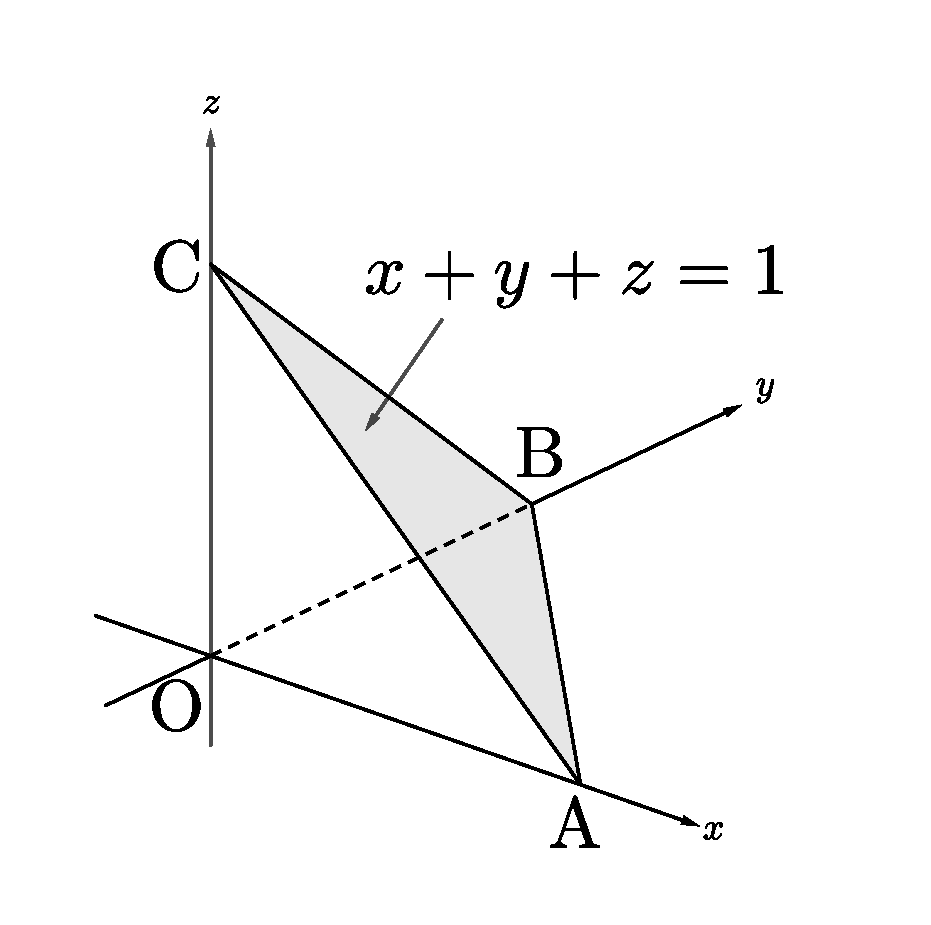
\includegraphics[height=6cm]{13/tetrahedron.pdf}
  \end{figure}
  
  \noindent 従って,$D=\Set{(x,y) \ \mid \ x+y \leqq 1, \; x \geqq
    0, \; y\geqq 0} \; \left(\subset \mathbb{R}^2\right)$ とすれば
  \[
    V = \Set{(x,y,z) \ \mid \ (x,y) \in D, \; 0 \leqq z \leqq 1-x-y}
  \]
  と書ける.よって,定理\ref{thm:iterated3}によって次のように計算できる.
  \[
    \begin{aligned}
      \iiint_{V} \frac{dxdydz}{(1+x+y+z)^3}
      &= \iint_{D}\left( \int_{0}^{1-x-y} \frac{dz}{(1+x+y+z)^3} \right) \ dx dy\\[1ex]
      &  = \iint_{D} \left[ -\frac{1}{2(1+x+y+z)^2} \right]_{z=0}^{z=1-x-y} \ dx dy\\[1ex]
      &  = \iint_{D}\left( \frac{1}{2(1+x+y)^2} - \frac{1}{8}\right) \ dx dy = \frac{1}{2}\log 2 - \frac{5}{16}
    \end{aligned}
  \]
\end{example}

\subsection{変数変換}

2重積分と同様に,適切な変数変換によってより計算しやすい3重積分に書き直せることがある.

\begin{theorem}
  変数変換
  \[
    x=\varphi(u,v,w), \; y=\psi(u,v,w), \; z=\chi(u,v,w) \quad (\varphi, \psi, \chi \text{ は $C^1$ 級})
  \]
  によって,$xyz$ 空間の $V$ と $uvw$ 空間の $W$ が1対1に対応し,$(u,v,w) \in W$ に対して
  \[
    J(u,v,w) := \left|
      \begin{array}{ccc}
        x_{u} & x_{v} & x_{w}\\
        y_{u} & y_{v} & y_{w}\\
        z_{u} & z_{u} & z_{w}
      \end{array}
    \right| \neq 0 \quad \left( J(u,v,w) \text{ は Jacobian と呼ばれる} \right)
  \]
  とする.このとき,3変数関数 $f$ が $V$ 上重積分可能なら以下が成り立つ.
  \begin{equation}\label{eq:trans-3d}
    \iiint_V f(x,y,z) \ dxdydz 
    = \iiint_W f\left( \varphi(u,v,w), \psi(u,v,w), \chi(u,v,w)\right) |J(u,v,w)|\ du dv dw
  \end{equation}
\end{theorem}

\begin{remark}
  2重積分のときと同様に,上の定理の条件はもう少し緩められる.例え
  ば,3次元の極座標変換
  \[
    x=r\cos \theta \cos \varphi, \; y=r\sin\theta \cos\varphi, \; z=r\sin\varphi
  \]
  はよく用いられる変数変換である.
  \begin{figure}[h]
    \centering
    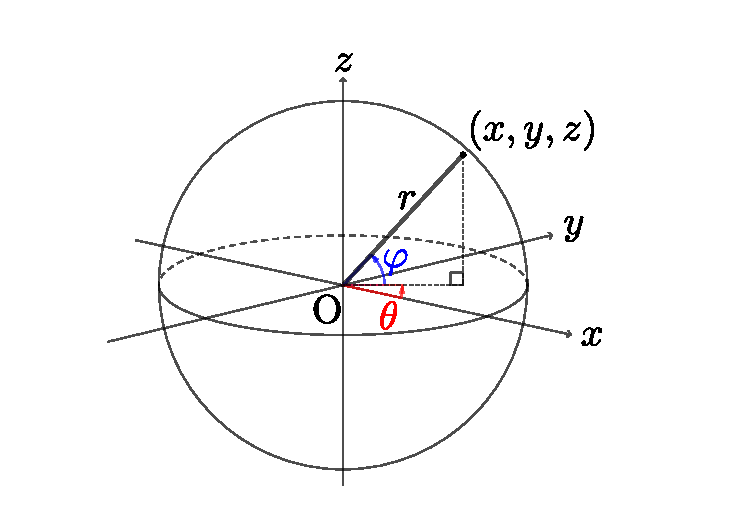
\includegraphics[height=5cm]{13/trans-pole3d.pdf}
  \end{figure}
  
  \noindent これは $r\theta\varphi$ 空間の
  \[
    W=\Set{(r,\theta,\varphi) | 0 \leqq r \leqq R, \, 0 \leqq \theta \leqq 2\pi, \;
      -\frac{\pi}{2} \leqq \varphi \leqq \frac{\pi}{2}}
  \]
  を $xyz$ 空間の $V=\Set{(x,y,z) | x^2+y^2+z^2=R^2}$ に変換する
  が,1対1の対応ではない.しかしながら,\uwave{$W$ から体積 $0$ の部分集合を適
    切に除けば1対1に対応する}.また,この変換の Jacobian は
  \[
    J(r, \theta, \varphi) = \left|
      \begin{array}{ccc}
        \cos \theta \cos \varphi & -r\sin\theta \cos\varphi & -r\cos\theta\sin\varphi\\
        \sin \theta \cos \varphi & r\cos\theta \cos\varphi & -r\sin\theta\sin\varphi\\
        \sin\varphi & 0 & r\cos\varphi
      \end{array}
    \right| = r^2\cos\varphi
  \]
  であるが,これも \uwave{$W$ から体積 $0$ の部分集合を適切に除いたとこ
    ろで $J \neq 0$ である}( 具体的には $W$ から部
  分集合 $\Set{(r, \theta, \varphi) \ \mid \ r=0 \text{ または }
    \cos \varphi=0}$ を除けばよい).この例のように,2つの波線部を満たしていれ
  ば(\ref{eq:trans-3d}) が成り立つ.
\end{remark}

\begin{example}\label{exmp:trans-pole3d}
  半径 $R \; (>0)$ の球
  $V=\Set{(x,y,z) \ \mid \ x^2+y^2+z^2 \leqq R^2}$ 上の次の3重積
  分を計算する.
  \[
    \iiint_V dx dy dz
  \]
  先ほど説明した通り,3次元の極座標変換
  \[
    x = r \cos\theta \cos \varphi, \quad y = r\sin\theta\cos\varphi,
    \quad z=r\sin\varphi
  \]
  によって,$r\theta\varphi$ 空間の
  \[
    W=\Set{((r,\theta,\varphi) \ \mid \ 0 \leqq r \leqq R, \; 0 \leqq
      \theta \leqq 2\pi, \; -\frac{\pi}{2} \leqq \varphi \leqq \frac{\pi}{2}}
  \]
  が $xyz$ 空間の $V$ に変換される.変換
  の Jacobian は
  \[
    J(r, \theta, \varphi) = \left|
      \begin{array}{ccc}
        \cos \theta \cos \varphi & -r\sin\theta \cos\varphi & -r\cos\theta\sin\varphi\\
        \sin \theta \cos \varphi & r\cos\theta \cos\varphi & -r\sin\theta\sin\varphi\\
        \sin\varphi & 0 & r\cos\varphi
      \end{array}
    \right| = r^2\cos\varphi
  \]
  なので,(\ref{eq:trans-3d}) を適用して次のように計算できる.
  \[
    \begin{aligned}
      \iiint_{V} dx dy dz
      &= \iiint_{W} |J(r, \theta, \varphi)| \ dr d\theta d\varphi
        = \left( \int_{0}^{R} r^2 \ dr\right) \left( \int_{0}^{2\pi} d\theta\right)
        \left( \int_{-\frac{\pi}{2}}^{\frac{\pi}{2}} \cos\varphi\ d\varphi\right) = \frac{4}{3}\pi R^3
    \end{aligned}
  \]
\end{example}

\subsection{3重積分と立体の体積}

平面図形 $D$ 上での定数関数 $1$ の2重積分 $\ds \iint_{D} dxdy$ が $D$ の面積に等しいのと同様に,以下が成り立つ.

\begin{theorem}\label{thm:3d-vol}
  定数関数が重積分可能な有界閉領域 $V \; (\subset \mathbb{R}^3)$ の体積は3重積分 $\ds \iiint_{V} dxdydz$ に等しい.\\
\end{theorem}

\begin{example}
  例\ref{exmp:trans-pole3d}で求めた3重積分は半径 $R$ の球 $V=\Set{(x,y,z) \ \mid \ x^2+y^2+z^2 \leqq R^2}$ の体積に等しい.\\
\end{example}

\begin{remark}
  3重積分は何を計算しているかを実感しづらいかもしれないが,一つの物理的な例として
  \begin{center}
    「密度の積分は物体の質量に等しい」
  \end{center}
  を挙げておく.空間にある物体 $V$ の点 $(x,y,z)$ での密度が $\rho(x,y,z)$ で与えられるなら,3重積分
  \[
    \iiint_{V} \rho(x,y,z) \ dx dy dz
  \]
  は $V$ の質量に等しい.特に密度が均一な,つまり $\rho(x,y,z)=1$ の物
  体はその質量と体積が等しい.これが定理\ref{thm:3d-vol}が成り立つ理由
  である.
\end{remark}

\newpage

\begin{example}\label{exmp:kantsu2}
  半径 $R>0$ の円柱2本が垂直に交わってできる共通部分(円柱貫通体)の体積を求める.

  \begin{figure}[h]
    \centering
    \begin{tabular}{cc}
      \includegraphics[height=6cm]{13/cylinders2.jpg}
      & \includegraphics[height=6cm]{13/kantsu2.jpg}
    \end{tabular}
  \end{figure}
  
  \noindent 定理\ref{thm:3d-vol}
  から,$V=\Set{(x,y,z) \ \mid \ x^2+y^2 \leqq R^2, \; y^2+z^2 \leqq
    R^2}$ として次の3重積分を計算すればよい.
  \[
    \iiint_{V} dx dy dz
  \]
  $D=\Set{(x,y) | x^2+y^2 \leqq R^2} \; ( \subset \mathbb{R}^2)$ とすれば,
  \[
    V=\Set{(x,y,z) \ \mid \  (x,y) \in D,  \;  -\sqrt{R^2-y^2} \leqq z \leqq \sqrt{R^2-y^2}}
  \]
  と書けるので,定理\ref{thm:iterated3}より次のように計算できる.
  \[
    \begin{aligned}
    \iiint_{V} \ dx dy dz  &= \iint_{D} \left( \int_{-\sqrt{R^2-y^2}}^{\sqrt{R^2-y^2}} dz\right) dx dy
          = \iint_{D} 2\sqrt{R^2-y^2} \ dx dy\\[1ex]
        &= 2\int_{-R}^{R}\sqrt{R^2-y^2} \left( \int_{-\sqrt{R^2-y^2}}^{\sqrt{R^2-y^2}} dx\right) dy
          = 4 \int_{-R}^{R} \left( R^2-y^2\right) dy = \frac{16}{3} R^2
    \end{aligned}
  \]
  この円柱貫通体という立体ははなかなか形を想像しづらいので,以下のリンク先で図形を
  回したり拡大縮小したり余計な柱を消したりしながら想像力を補ってください.
  \begin{figure}[h]
    \centering
    \includegraphics[height=3cm]{13/QR_cylinders2.png}\\
    \url{https://www.geogebra.org/m/jd93vtj8}
  \end{figure}
\end{example}

\newpage

\subsection{練習問題}

\begin{enumerate}

  \setlength{\itemsep}{1zh}
  
\item 次の3重積分を計算しよう.

  \vspace{1zh}

  \begin{enumerate}[(1)]
    \setlength{\itemsep}{1zh}
    
  \item $\ds \iiint_{V} y \ dx dy dz \qquad V=\Set{(x,y,z) \ \mid \
      x+y \leqq 1, \; 0 \leqq x, \; 0 \leqq y, \; 0 \leqq z \leqq x}$

  \item $\ds \iiint_{V} x \ dx dy dz \qquad V=\Set{(x,y,z) \ \mid \
      0 \leqq x \leqq y \leqq 1, \; 0 \leqq z \leqq x+y}$

  \item $\ds \iiint_{V} xz \ dx dy dz \qquad V=\Set{(x,y,z) \ \mid \
      0 \leqq z \leqq 1-x^2-y^2}$

  \item  $\ds \iiint_{V} xy \ dx dy dz \qquad V=\Set{(x,y,z) \ \mid \
      x+y+z \leqq 1, \; 0 \leqq x, \; 0 \leqq y, \; 0 \leqq z}$

  \item $\ds \iiint_{V} x^2 \ dx dy dz \qquad V=\Set{(x,y,z) \ \mid \
      |x| + |y| + |z| \leqq 1}$ 
  \end{enumerate}

\item いい感じに変数を変換して次の3重積分を計算しよう.

  \vspace{1zh}

  \begin{enumerate}[(1)]

    \setlength{\itemsep}{1zh}
    
  \item $\ds \iiint_{V} (x+y)(y+z)(z-3x) \ dx dy dz \qquad V=\Set{(x,y,z) \ | \
      \begin{array}{l}
        0 \leqq x+2y \leqq 1, \; 0 \leqq y+z \leqq 2,\\
        0 \leqq z-3x \leqq 1
      \end{array}}$
    
  \item $\ds \iiint_{V} \sqrt{x^2+y^2+z^2} \ dx dy dz \qquad V=\Set{(x,y,z) \ \mid \
      x^2+y^2+z^2 \leqq 1}$

  \item $\ds \iiint_{V} \sqrt{1-x^2-y^2-z^2} \ dx dy dz \qquad V=\Set{(x,y,z) \ \mid \
      x^2+y^2+z^2 \leqq 1}$

  \item $\ds \iiint_{V} x \ dx dy dz \qquad V=\Set{(x,y,z) \ \mid \
      x^2+y^2+z^2 \leqq 1, \; 0 \leqq x, \; 0 \leqq y, \; 0 \leqq z}$

  \item $\ds \iiint_{V} z \ dx dy dz \qquad V=\Set{(x,y,z) \ \mid \
      x^2+y^2+z^2 \leqq 1, \; x^2+y^2 \leqq x, \; 0 \leqq z}$
  \end{enumerate}

\item 半径 $R \; (>0)$ の円柱3本が互いに垂直に交わってできる以下の立
  体 $V$ の体積を求めよう.
  \[
    V=\Set{(x,y,z) \ \mid \ x^2+y^2 \leqq R^2, \; y^2+z^2 \leqq R^2, \; z^2+x^2 \leqq R^2}
  \]
  例\ref{exmp:kantsu2}と同様にこの立体も円柱貫通体と呼ばれる.立体的な図は以下
  のリンク先でご確認ください.
  \begin{figure}[h]
    \centering
    \includegraphics[width=2cm]{13/QR_cylinders3.png}\\
    \url{https://www.geogebra.org/m/xaswsqpu}
  \end{figure}
\end{enumerate}

\begin{figure}[b]
  答え:{\small 1. (1) $\frac{1}{24}$ \; (2) $\frac{5}{24}$ \; (3) $0$
  \; (4) $\frac{1}{120}$ \; (5) $\frac{2}{15}$ \quad
  2. (1) $\frac{1}{10}$ \; (2) $\pi$ \; (3) $\frac{\pi^2}{4}$ \;
  (4) $\frac{\pi}{16}$ \; (5) $\frac{5\pi}{64}$ \quad 3. $(16-8\sqrt{2})R^3$}
\end{figure}

\end{document}
